% Histórico da kdtree:
%  - primeira proposta.
%  - Objetivo. Eficientcia
%  - Teste de colisão, pertinencia e amplitude
% Utilizacao:


% Intro a indexacao (motivacao):
% - principal funcionalidade do algoritmo (comparacao de dominancia)
% - acaba sendo o gargalo da aplicacao, pois as outras operações são lineares
%     com o tamanho do conjunto de solucoes
% - porem esta operacao pode ser otimizada se as solucioes estiverem
%     propriamente indexadas
The main operation in Algorithm~\ref{alg:bazgan} is
filtering all partially efficient solutions
from the early generated set (line 7).
Ensuring that a partial solution has no dominant
may demand quadratic effort on the total number of solutions
if implemented as pairwise comparison.
This operation tends to be the computational bottleneck of the algorithm
since it is executed on every stage
and all others operations have linear computational complexity.
For this reason the optimization of this operation
is crucial for an efficient algorithm.

If solutions are mapped into points in a multi-dimensional space,
it can be deduced from equation~(\ref{eq:kdom}) that
this operation corresponds on checking whether a point exists in a certain region.
Formally:
\begin{align*}
    \text{ if } \; &\domk{y}{x} \; \text{ then } \; \pnt{y} \in R(\sol{x}) \\
  \text{where} \phantom{mmmmm} \\
    \pnt{x} &= \big(\obj{1}{x}, \ldots, \obj{\np}{x}, \weight{x}\big) \\
    R(\sol{x}) &= \left\{ a \in \mathbb{R}^{\np+1} \;\middle|\;
      a_{\np+1} \leq \weight{x}
      \, \text{ and } \,
      a_i \geq \obj{i}{x}, \; i \in \{1, \ldots, \np\}
      \right\}
\end{align*}

The problem of determining whether a point exists in a certain region
of space is known in geometric computation as
\emph{range search}\cite{agarwal1999geometric}
and is usually solved with the use of a
\kdtree{}\cite{preparata2012computational}.
The \kdtree{} is a type of binary search tree for indexing multi-dimensional
data with simple construction and low space usage.
Despite its simplicity, it efficiently supports nearest
neighbour search and range search operations~\cite{bentley1975} and
for those reasons \kdtree{} is widely used on
spacial geometry algorithms~\cite{preparata2012computational, guttman1984r},
clustering~\cite{kanungo2002efficient, indyk1998approximate}
and graphic rendering algorithms~\cite{owens2007survey}.

Like a standard binary search tree, the \kdtree{} subdivides data at each
recursive level of the tree.
Unlike a standard binary tree, that uses only one key for all levels of the tree,
the \kdtree{} uses $k$ keys and cycles through these keys for successive levels
of the tree.
Figure~\ref{fig:kdom-kd} presents
(a) points on a plane
indexed by a (b) \dtree{2}.
The first and third level of the \dtree{2} indexes $x$ component
while second level indexes $y$ component.
Each point branches a subregion in two -- showed on the figure by a
thicker line -- according to the component being indexed.

\begin{figure}[H]
  \centering
  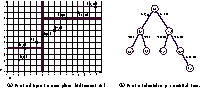
\includegraphics[scale=3.8]{src/imgs/dom-kd}
  \caption{Example of points indexed in a \kdtree{}.}
  \label{fig:kdom-kd}
\end{figure}

Figure~\ref{fig:query} presents an example of dominance check operation with indexed
solutions using a \dtree{2}.
The gray area has no intersection with the dominant (cross-hatched) area, therefore
solutions inside it are not evaluated.
The efficiency of this pruning action grows
with the amount of points.

\begin{figure}[H]
  \centering
  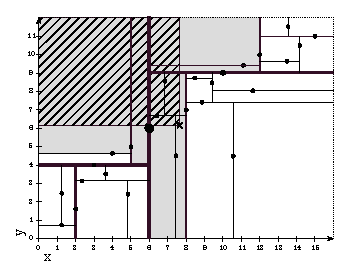
\includegraphics[scale=1.7]{src/imgs/query}
  \caption{Example of dominance check operation using \kdtree{} for solution indexing.}
  \label{fig:query}
\end{figure}

% Discussão sobre eficiencia da kdtree em relação ao número de dimensões:
Concerning the efficiency of the \kdtree{}, it is important to
consider the number of dimensions it is indexing.
As a general rule, a \kdtree{} is suitable for the efficiently indexing of $n$ elements
if $n$ is much greater than $2^k$.
Otherwise, when \kdtree{} is used with high-dimensional data, most of the elements
in the tree will be evaluated and the efficiency is no better than exhaustive search~\cite{toth2004handbook}.

The use of \kdtree{} is applied on Algorithm~\ref{alg:bazgan}
to index sets for which there is a demand of dominance check operation.
These sets are (a) the set $\solSett^k$ of intermediate partial solutions
and (b) the set of upper bound solutions.
In both cases there is no need to evaluate the weight of the solution,
therefore a \kdtree{} indexing up to all $\np$ objective values may be used.

It is expected that the use of a \kdtree{}
assists the dominance check operation by
pruning a larger amount of points than a single dimensional indexing,
which may demand a smaller number of solution evaluation,
thus increasing the algorithm performance.